\documentclass[border=2pt]{standalone}
\usepackage{tikz}
\usetikzlibrary{arrows.meta,chains,%
                    decorations.pathreplacing}
\usetikzlibrary{matrix,positioning,arrows.meta,arrows}

\tikzset{
mymat/.style={
  matrix of nodes,
  nodes in empty cells,
  text height=2.5ex,
  text depth=0.75ex,
  text width=3.25ex,
  align=center,
  column sep=-\pgflinewidth
  }
}
\tikzset{
  rows/.style 2 args={
    sub@rows/.style={row ##1 column #2/.style={nodes={rectangle,draw=black}}},
    sub@rows/.list={#1}
  },
  box/.style 2 args={
    sub@box/.style={rows={#1}{##1}},
    sub@box/.list={#2}
  }
}
\begin{document}

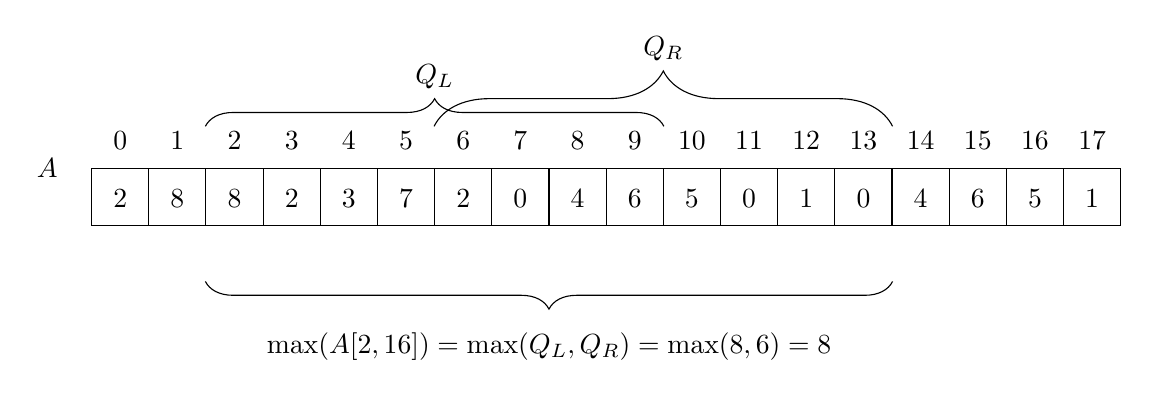
\begin{tikzpicture}[>=latex]
\matrix[mymat,anchor=west,
    box={2}{1, 2, 3, 4, 5, 6, 7, 8, 9, 10, 11, 12, 13, 14, 15, 16, 17, 18}]
at (0,0) 
(mat1)
{ 
  0 & 1 & 2 & 3 & 4 & 5 & 6 & 7 & 8 & 9 & 10 & 11 & 12 & 13 & 14 & 15 & 16 & 17 \\
  2 & 8 & 8 & 2 & 3 & 7 & 2 & 0 & 4 & 6 &  5 &  0 &  1 &  0 &  4 &  6 &  5 &  1  \\};

\node[left=5pt of mat1]
{
   $A$ \\
};

\draw[decorate,decoration={brace, amplitude=10pt, raise=20pt, mirror}]
  (mat1-2-3.south west) to node[black,midway,below= 35pt] {$\max(A[2, 16]) = \max(Q_L, Q_R) = \max(8, 6) = 8$} (mat1-2-14.south east);

\draw[decorate,decoration={brace, amplitude=10pt, raise=15pt}]
  (mat1-2-3.north west) to node[black,midway,above=25pt] {$Q_L$} (mat1-2-10.north east);

\draw[decorate,decoration={brace, amplitude=20pt, raise=15pt}]
  (mat1-2-7.north west) to node[black,midway,above=35pt] {$Q_R$} (mat1-2-14.north east);
\end{tikzpicture}

\end{document}